\documentclass[10pt,a4paper]{article}
\usepackage[utf8]{inputenc}
\usepackage[italian]{babel}
\usepackage{amsmath}
\usepackage{amsfonts}
\usepackage{float}
\usepackage{caption}
\usepackage{subcaption}
\usepackage{adjustbox}
\usepackage{amssymb}
\usepackage[separate-uncertainty = true]{siunitx}
\usepackage{graphicx}
\usepackage[left=2cm,right=2cm,top=2cm,bottom=2cm]{geometry}
\usepackage{booktabs}
\newcommand{\rem}[1]{[\emph{#1}]}
\newcommand{\exn}{\phantom{xxx}}

\author{Giulio Cordova}
\title{Esperienza preliminare}
\begin{document}
\twocolumn
\date{\today}
\maketitle

\section{Scopo dell'esperienza}

Lo scopo dell'esperienza preliminare è di familiarizzare con alimentatori di alta tensione, segnali dai fotomoltiplicatori, cavi (Linee di trasmissione) coassiali, oscilloscopi, discriminatori, unità di coincidenza e contatori, nonché determinare l'efficienza dei rivelatori dei raggi cosmici, in particolare al variare della tensione di alimentazione dei tubi fotomoltiplicatori (PMT).

\section{Descrizione del setup}

Il setup consiste in varie lastre scintillanti di spessore \SI{2}{\centi\meter} e area di circa \SI{1872}{\centi\meter\squared} connessi a tubi fotomoltiplicatori alimentati da un generatore di alta tensione. L'uscita dei fotomoltiplicatori è connessa a un Rack NIM che all'interno contiene
\begin{itemize}
    \item un'unità discriminante CAEN N84;
    \item due moduli di coincidenza CERN N6234;
    \item un contatore INFN Multiscaler 130.
\end{itemize} 
Per la lettura del segnale è utilizzato un oscilloscopio Textronik 2012, nonché cavi coassiali di lunghezza differente a connettori LEMO e BNC. Si ha infine un multimetro utilizzato per leggere la soglia in tensione del trigger del discriminatore.

Un disegno schematico del setup è raffigurato in Figura \ref{fig:setup}, dove si è omessa volontariamente la postazione computer che consente di regolare i voltaggi dei generatori di alta tensione. In Figura \ref{fig:setup} è riportato anche uno schema della geometria di una lastra scintillante con la relativa connessione al fotomoltiplicatore.



\begin{figure}[h]
    \centering
    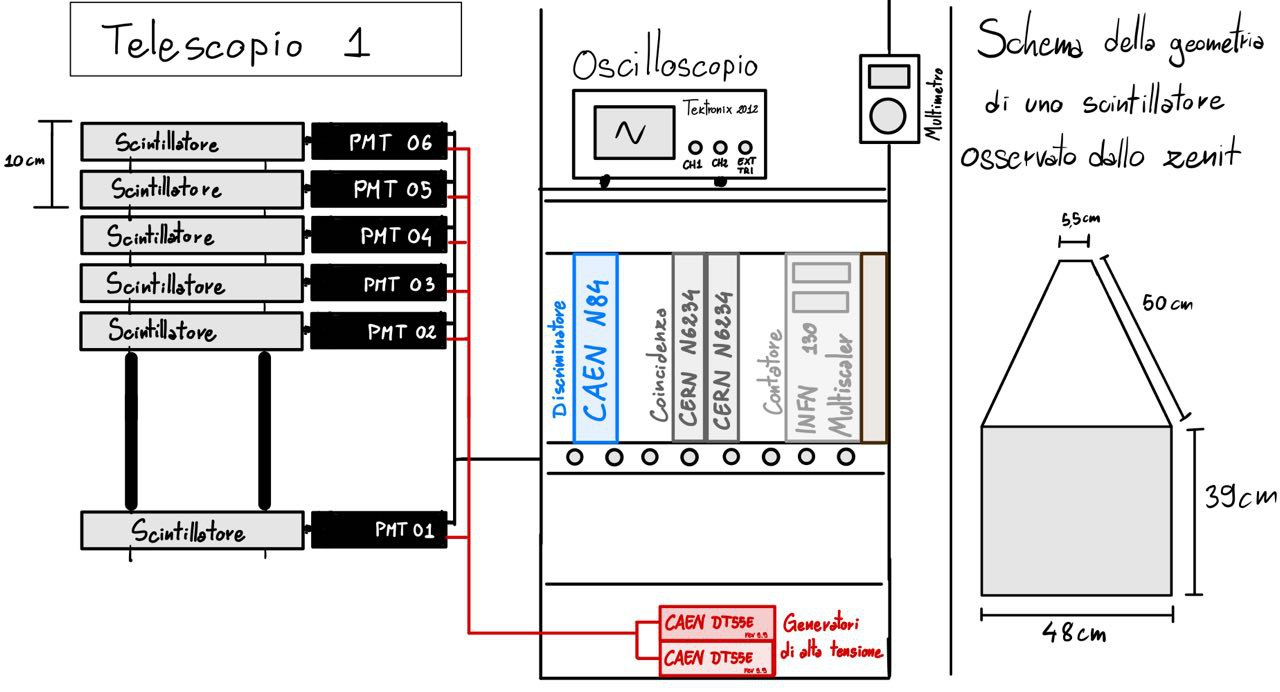
\includegraphics[width=\columnwidth]{img/setup+.jpeg}
    \caption{Setup dell'eseperimento alla postazione Telescopio 1 e schema geometrico di una lastra scintillante}
    \label{fig:setup}
\end{figure}


\section{Misure preliminari}

Come prima cosa si è collegato il segnale del fotomoltiplicatore più alto (PMT06 in Figura \ref{fig:setup}) al primo ingresso dell'oscilloscopio. Poiché l'impedenza interna dell'oscilloscopio è di $Z_{osc}=\SI{1}{\mega \ohm}$, si è terminato il cavo coassiale con la sua impedenza interna di $Z_{cavo}=\SI{50}{\ohm}$, al fine di evitare effetti di riflessione.

\subsection{Tensione di alimentazione del PMT}

Impostando il trigger sul canale 1 per un segnale a rampa negativa di almeno $V_{trig}=\SI{-40}{\milli \volt}$, si è andato ad alimentare gradualmente il primo tubo a fotomoltiplicatore, annotando la frequenza di trigger. Si è notato che fino a $V_1=\SI{1600}{\volt}$ la frequenza rimaneva minore di  $\nu_{trig}=\SI{10}{\hertz}$, mentre al di sopra di $V_1=\SI{1750}{\volt}$ inizia ad oscillare fra decine di Hertz e il valore ricercato di $\nu_{trig}=\SI{100}{\hertz}$. Questa condizione sulla frequenza di trigger si è raggiunta con maggior stabilità a una tensione di alimentazione pari a $V_1=\SI{1775}{\volt}$. 
%inserire screenshot dell'oscilloscopio, magari uno per trigger alto e uno per trigger basso
    Lasciando fissa la tensione di alimentazione del PMT si può osservare come varia la frequenza di trigger al variare della soglia in tensione $V_{trig}$. Non è stato chiaro come prendere il dato della frequenza di trigger, in quanto la lettura dell'oscilloscopio riguardo quest'ultimo dato non è fissa ma oscilla tra valori distanti fra loro anche di decine di Hertz. Si è scelto quindi di lasciare l'oscilloscopio alla stessa soglia per diversi secondi e registrare la media fra il valore più alto e quello più basso osservato. L'incertezza sulla tensione di soglia di trigger è stata valutata consultando il datasheet dell'oscilloscopio ($\pm0.2 \text{div} \cdot \text{V}/\text{div}$), mentre per quanto riguarda la frequenza di trigger si è stimata prendendo la distanza dai valori massimi/minimi osservati, dove si è registrato 0 quando la frequenza risultava minore di \SI{10}{\hertz}. I dati sono riportati in Tabella \ref{tab:freq} e Figura \ref{fig:freq}. Quest'ultima suggerisce inoltre un comportamento ovvio, ovvero che abbassando la soglia in tensione del trigger, l'oscilloscopio mostra eventi che producono una caduta di potenziale minore, portando pertanto la frequenza di eventi triggerati ad aumentare.

\begin{table}[h]
    \centering
\begin{tabular}{c|c}
Soglia [mV] & Frequenza [Hz] \\
\midrule
-190±10 &      9.0±9.0 \\
-180±10 &    12.5±12.5 \\
-170±10 &    14.5±14.5 \\
-160±10 &    23.0±23.0 \\
 -150±4 &    35.0±22.0 \\
 -140±4 &    38.5±25.5 \\
 -130±4 &    39.5±23.5 \\
 -120±4 &    43.0±24.0 \\
 -110±4 &    50.0±26.0 \\
 -100±4 &    69.0±41.0 \\
  -90±2 &    68.0±34.0 \\
  -80±2 &    77.5±34.5 \\
  -70±2 &    95.0±48.0 \\
  -60±2 &   103.5±55.5 \\
  -50±2 &   110.0±65.0 \\
  -40±2 &   200.5±69.5 \\
  -30±1 & 1380.0±140.0 \\
  -20±1 & 4300.0±400.0 \\
  -15±1 & 5800.0±330.0 \\
  -10±1 & 7000.0±500.0 \\
\end{tabular}


    \caption{Dati relativi alla frequenza di trigger in funzione della soglia in voltaggio del trigger. Questi dati sono stati usati per creare la Figura \ref{fig:freq}}
    \label{tab:freq}
\end{table}

\begin{figure}[h]
    \centering
    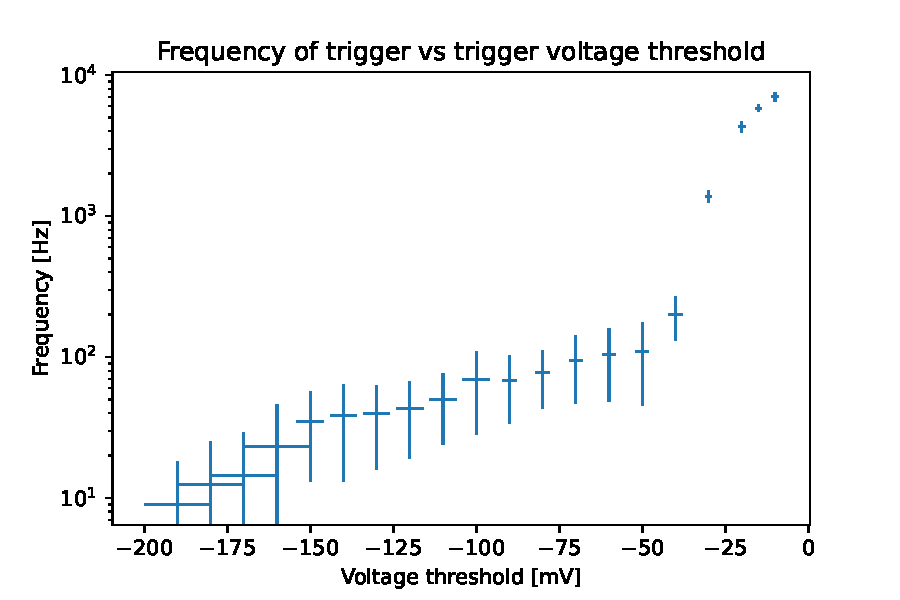
\includegraphics[width=\columnwidth]{../img/trigger.pdf}
    \caption{Frequenza di trigger vs soglia di tensione del trigger}
    \label{fig:freq}
\end{figure}


\subsection{Ritardo dell'unità discriminante}\label{ritardo}
Successivamente si è connessa l'unità discriminante mandando in ingresso il segnale del PMT, assicurandosi che la soglia di discriminazione fosse la stessa del trigger dell'oscilloscopio $V_{trig=}\SI{-40}{\milli \volt}$. Questo valore è stato regolando agendo sul trimmer del discriminatore con una lettura su un multimetro digitale. è utilizzato un multimetro per misurare  Dal momento che i due ingressi del discriminatore sono cortocircuitati, è possibile continuare a vedere il segnale del PMT all'oscilloscopio collegando questo al secondo ingresso dell'unità discriminante. Il discriminante ha una impedenza di ingresso di $Z_{ing,dis}=\SI{2}{\kilo\ohm}$, pertanto il cavo coassiale necessita di essere terminato alla sua impedenza interna $Z_{cavo}=\SI{50}{\ohm}$. Tuttavia, l'ingresso dell'unità discriminata è cortocircuitato e si utilizza un ulteriore cavo per mandare il segnale all'oscilloscopio, pertanto è sufficiente una sola terminazione del cavo all'ingresso dell'oscilloscopio. Anche l'uscita del discriminatore viene collegata all'oscilloscopio con la solita terminazione, in modo da osservare la tipica caduta di potenziale di durata variabile al momento della presenza di un segnale discriminato, mostrato in Figura \ref{fig:discr}.

\begin{figure}[h]
    \centering
    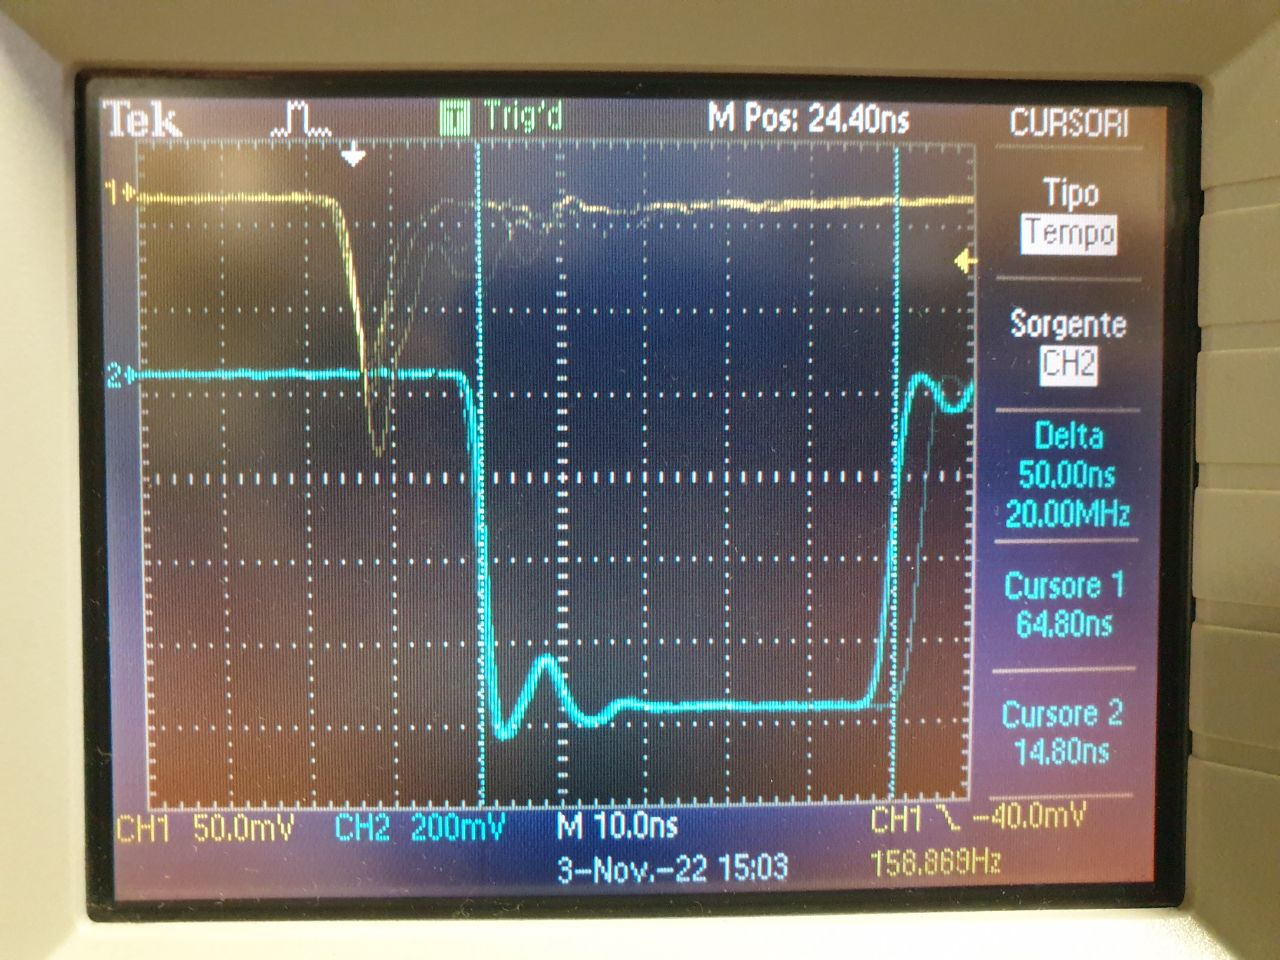
\includegraphics[width=0.8\columnwidth]{img/discriminato.jpeg}
    \caption{Segnale discriminato nel canale 2 (blu). Si noti la lunghezza del segnale impostata su \SI{50}{\nano\second}}
    \label{fig:discr}
\end{figure}

All'oscilloscopio si osserva come questi due segnali non siano contemporanei ma che è presente un ritardo introdotto dall'unità discriminante. Al fine di valutare quest'ultimo minimizzando l'errore, si procede a misurare la distanza dei due segnali nel momento di massima pendenza della caduta di potenziale, stimata a metà altezza del picco negativo massimo. Si misura quindi sia per il segnale del PMT che per quello del discriminatore il valore di massima caduta di potenziale, rispettivamente a $V_{PMT}=\SI{-70}{\milli \volt}$ e $V_{discr}=\SI{-856}{\milli \volt}$. Misurando quindi con i cursori la distanza temporale fra il punto a $\frac{1}{2}V_{PMT}=\SI{-35}{\milli \volt}$ del segnale del PMT e del punto a $\frac{1}{2}V_{discr}\SI{-428}{\milli \volt}$ del segnale discriminato, si stima un ritardo di $t_{rit}=\SI{15}{\nano \second}$. A questo si deve aggiungere il ritardo indotto dai cavi utilizzati. Per entrambi i segnali osservati all'oscilloscopio si ha che questi sono collegati ai PMT con:

\begin{itemize}
    \item un cavo con $t_{rit, cavo1}=\SI{10}{\nano \second}$ che collega il PMT al Rack NIM (comune ad entrambi i segnali);
    \item un cavo con $t_{rit, cavo2}=\SI{2}{\nano \second}$ che collega il canale di lettura sul rack al discriminatore (comune a entrambi i segnali);
    \item un cavo con $t_{rit, cavo2}=\SI{2}{\nano \second}$ che collega il secondo ingresso del discriminatore al primo canale dell'oscilloscopio (ingresso del segnale PMT);
    \item un cavo con $t_{rit, cavo2}=\SI{2}{\nano \second}$ che collega l'uscita del discriminatore al secondo canale dell'oscilloscopio (ingresso del segnale discriminato).
\end{itemize} 
Il ritardo complessivo dell'osservazione del segnale discriminato all'oscilloscopio rispetto al momento della rivelazione sarà quindi dato da

\[t_{tot}=t_{rit}+t_{rit, cavo1}+2t_{rit, cavo2}=\SI{29}{\nano \second}\]

mentre il ritardo del segnale del canale 1 rispetto alla rivelazione del segnale sarà dovuto solo ai cavi, quindi \[t_{rit, cavo}=t_{rit, cavo1}+2t_{rit, cavo2}=\SI{14}{\nano \second}\]
Poiché i segnali in ingresso all'oscilloscopio sono collegati entrambi con un cavo della stessa lunghezza, il ritardo misurato di $t_{rit}=\SI{15}{\nano \second}$ è effettivamente il ritardo indotto dall'unità di coincidenza senza ulteriori effetti di ritardo del cavo. \\
Prima di procedure ulteriormente ci si è accertati che la durata del segnale discriminato fosse di $T_{discr}=\SI{50}{\nano \second}$.

\subsection{Conteggi al variare della tensione di alimentazione}
In questa sezione si sono collegati i due rivelatori sottostanti al primo (PMT 05 e PMT 04 in Figura \ref{fig:setup}) con la stessa configurazione descritta nelle sezioni precedenti. Per linearità di esposizione, si è deciso di rinominare questi PMT1, PMT2, PMT3, ordinandoli dal più alto al più basso (in Figura \ref{fig:setup} PMT06, PMT05, PMT04 rispettivamente). 

Si collega inoltre alle uscite del discriminatore i canali del modulo di conteggio, ponendo attenzione ad utilizzare cavi della stessa lunghezza (\SI{3}{\nano \second}) per non introdurre un ritardo diverso per i tre rivelatori. Si procede quindi a investigare la variazione del numero di conteggi rispetto alla tensione di alimentazione dei fotomoltiplicatori, dove come incertezza si è ricavato dal datasheet $\epsilon_V=\pm0.05\% \text{ of read } \pm1 \text{ V}$. Per quanto riguarda l'errore sui conteggi si è presa la radice nel numero stesso, in quanto si è supposto che questi distribuicano come una Poisson.
In un intervallo di 100 secondi, si registrano i dati riportati in Tabella \ref{tab:counts}.
\begin{table}[h]
    \centering
    \adjustbox{max width=\columnwidth}{%
\begin{tabular}{c|c|c|c}
Tensione [V] &  Counts 1 &  Counts 2 &   Counts 3 \\
\midrule
           1500±2 &       0±0 &       4±2 &       12±3 \\
           1525±2 &       1±1 &      11±3 &       27±5 \\
           1550±2 &       6±2 &      31±6 &     177±13 \\
           1575±2 &       9±3 &      63±8 &     581±24 \\
           1600±2 &      31±6 &    182±13 &    1298±36 \\
           1625±2 &      63±8 &    292±17 &    1933±44 \\
           1650±2 &    186±14 &    485±22 &    2849±53 \\
           1675±2 &    364±19 &    826±29 &    5438±74 \\
           1700±2 &    601±25 &   1111±33 &  23432±153 \\
           1725±2 &    874±30 &   1883±43 &  60412±246 \\
           1750±2 &   2077±46 &   4549±67 &  91147±302 \\
           1775±2 & 10979±105 &   7787±88 & 118266±344 \\
           1800±2 & 31783±178 & 10069±100 & 139454±373 \\
           1825±2 & 50880±226 & 10793±104 & 164339±405 \\
           1850±2 & 62821±251 & 11703±108 & 188011±434 \\
           1875±2 & 69648±264 & 12665±113 & 231435±481 \\
           1900±2 & 74396±273 & 13281±115 & 274960±524 \\
           1925±2 & 77031±278 & 14377±120 & 344724±587 \\
           1950±2 & 80927±284 & 15775±126 & 485614±697 \\
           1975±2 & 88259±297 & 17174±131 & 663856±815 \\
\end{tabular}
}

    \caption{Conteggi in 100 secondi dei tre rivelatori al variare della tensione di alimentazione}
    \label{tab:counts}
\end{table}

Riportando i dati in un grafico si ottiene la Figura \ref{fig:counts}

\begin{figure}[h]
    \centering
    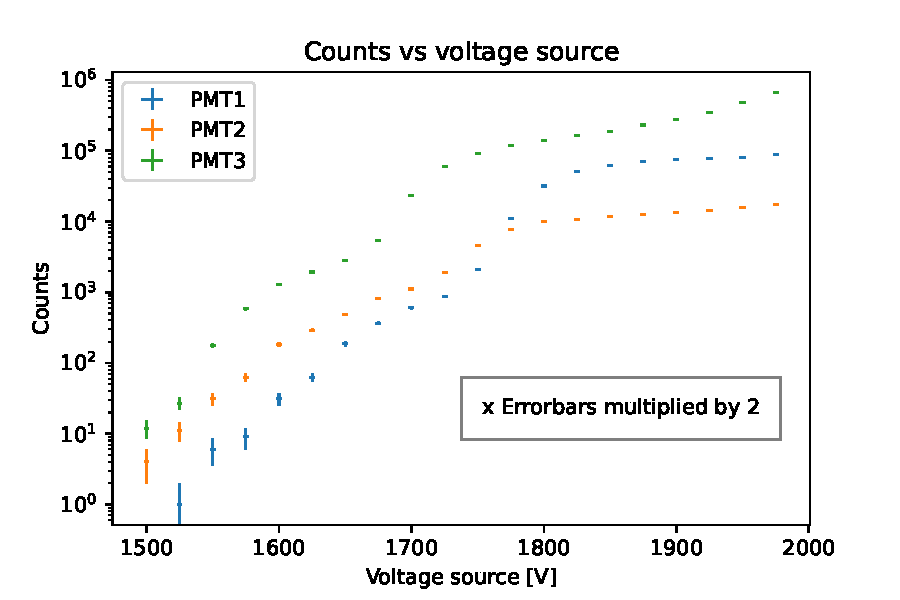
\includegraphics[width=0.8\columnwidth]{img/counts123_new.pdf}
    \caption{Conteggi dei tre rivelatori in funzione della tensione di alimentazione, dai dati della Tabella \ref{tab:counts}}
    \label{fig:counts}
\end{figure}

Come si può notare dalla figura, i tre rivelatori hanno una dipendenza diversa dalla tensione di alimentazione. In particolare, si nota come il terzo rivelatore abbia una dipendenza più marcata e cresca più velocemente rispetto agli altri. I dati in Tabella \ref{tab:counts} suggeriscono un ulteriore effetto, ovvero che il secondo fotomoltiplicatore raggiunge una sorta di plateau sorpassata una soglia di tensione di alimentazione individuata intorno ai $V_{plateau}=\SI{1800}{\volt}$. Non si tratta di un vero plateau in quanto i conteggi continuano ad aumentare al crescere della tensione, ma il rate di crescita si riduce drasticamente anche in confronto agli altri rivelatori. L'effetto non è ben visibile in scala logaritmica, pertanto si procede alla creazione di ulteriori grafici in scala lineare, riportati in Figura \ref{fig:counts_sep}. Si è deciso di andare a confrontare il primo e il secondo in Figura \ref{fig:counts_12} e riportare l'andamento del terzo in Figura \ref{fig:counts_3}, in quanto le scale dei due grafici sono molto diverse l'una dall'altra, rendendo l'effetto non visibile.

\begin{figure}[h]
\begin{subfigure}{.48\columnwidth}
  \centering
  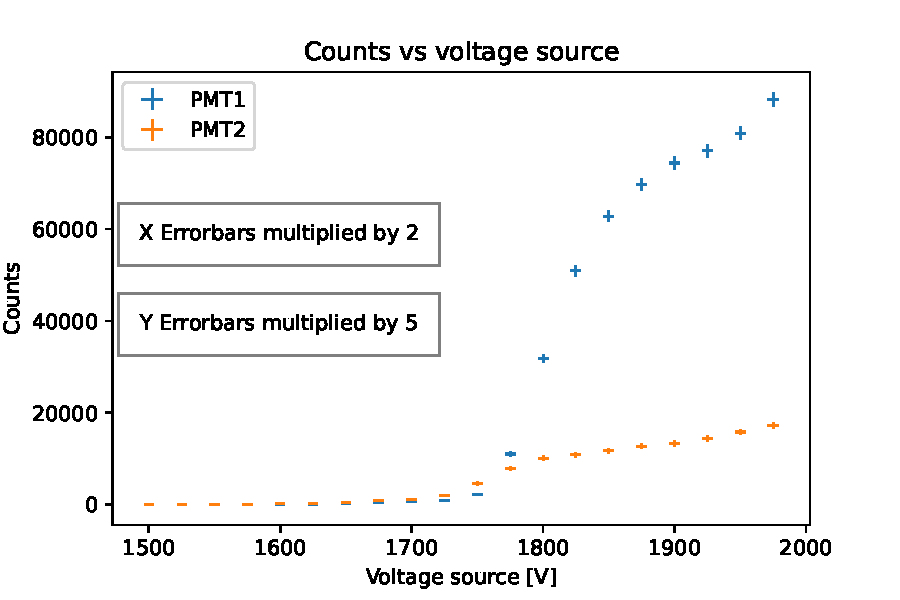
\includegraphics[width=\linewidth]{img/counts12_new.pdf}
  \caption{Primo e secondo}
  \label{fig:counts_12}
\end{subfigure}%
\hfill
\begin{subfigure}{.48\columnwidth}
  \centering
  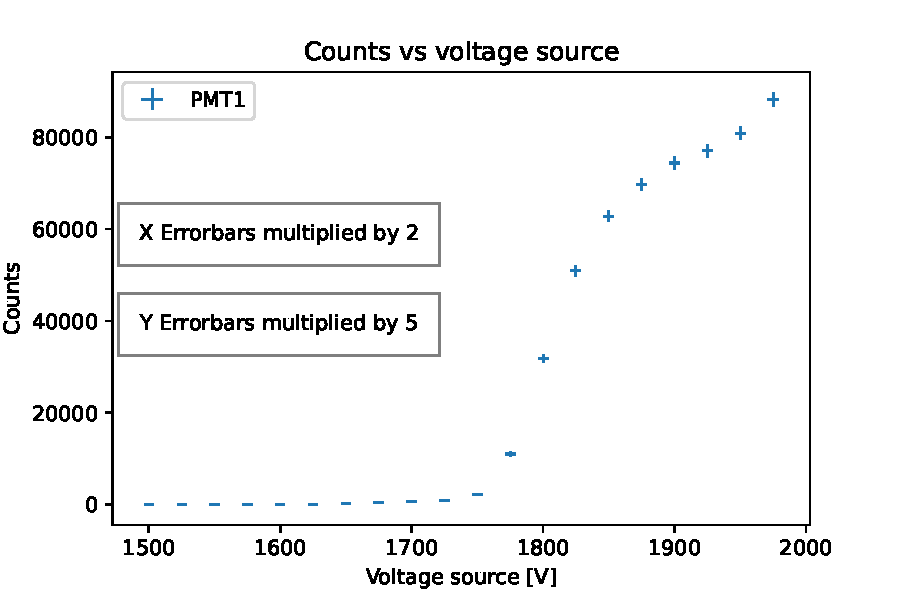
\includegraphics[width=\linewidth]{img/counts1_new.pdf}
  \caption{Terzo rivelatore}
  \label{fig:counts_3}
\end{subfigure}
\caption{Conteggi in vista separata dei dati della Tabella \ref{tab:counts}}
\label{fig:counts_sep}
\end{figure}

In Figura \ref{fig:counts_12} si nota molto bene l'effetto di simil-plateau, soprattutto se messo in relazione ai conteggi del primo rivelatore. La Figura \ref{fig:counts_3} suggerisce invece in modo evidente l'andamento dei conteggi con una potenza piuttosto elevata. 

\section{Misura dell'efficienza dei rivelatori}
Si procede quindi a settare le tensioni di alimentazione in modo tale che i tre rivelatori producano dei conteggi simili. In particolare si sceglie
\[ V_1=\SI{1790}{\volt} \quad\quad V_2=\SI{1850}{\volt} \quad\quad V_3=\SI{1700}{\volt} \]

Si inserisce adesso l'ultimo modulo, ovvero l'unità di coincidenza, che permetterà di determinare l'efficienza dei rivelatori. Al fine di prendere confidenza con questo modulo, si collegano agli ingressi A e B della coincidenza le uscite del primo e del secondo discriminatore, osservando all'oscilloscopio le uscite LIN e OUT del modulo di coincidenza. La prima restituisce un segnale della durata della coincidenza dei due segnali, mentre la seconda produce un singolo impulso di lunghezza fissa ogni volta che registra una coincidenza. Per una maggior accuratezza, è stato deciso di usare l'uscita LIN. % inserire figura dell'oscilloscopio dei due segnali

Con il metodo descritto nella sezione \ref{ritardo} si va a misurare il ritardo introdotto dall'unità di coincidenza per entrambe le uscite. In particolare, si misura

\[t_{LIN}=\SI{7.2}{\nano \second} \qquad t_{OUT}=\SI{12}{\nano\second} \]

Si monta adesso una seconda unità di coincidenza a cui si collegano agli ingressi A, B, C le uscite dei tre discriminatori, e si aggiunge anche l'uscita del terzo discriminatore all'ingresso C del primo modulo di coincidenza. Questo setup serve per far determinare le coincidenze doppie al primo modulo di coincidenza andando a spegnere ed accendere gli switch A, B e C, mentre il secondo modulo di coincidenza determina le coincidenze triple lasciando on tutti e tre gli switch. 

Lasciando le tensioni di alimentazione del PMT1 e del PMT3 costanti, si è proceduto a registrare il numero di conteggi di doppie e triple al variare della tensione di alimentazione del PMT2, al fine di valutare l'efficienza, definita in Eq. \eqref{eff}.

\begin{equation}
    \varepsilon=\frac{\# Triple}{\# Doppie}=\frac{N_t}{N_d}\label{eff}
\end{equation}

Questa definizione si basa sull'assunzione che una particella che passa dai rivelatori 1 e 3 sia passata anche dal secondo. Il numero delle triple può essere quindi essere quindi considerato distribuito con una binomiale, dove la probabilità di osservare una particella in coincidenza tripla rappresenta l'efficienza del secondo rivelatore. Questo modello è particolarmente utile per dare una stima dell'incertezza dell'efficienza dove si è supposto che non ci sia errore sulle doppie in quanto rappresentano il 100\% dei campionamenti, come derivato in Eq. \eqref{sigma}.

\begin{align}
    &Var(N_t)=N_d\varepsilon(1-\varepsilon)\\
    &\Longrightarrow \sigma\biggl(\frac{N_t}{N_d}\biggr)=\frac{\sqrt{N_d\varepsilon(1-\varepsilon)}}{N_d}=\sqrt{\frac{\varepsilon(1-\varepsilon)}{N_d}}\label{sigma}
\end{align}




Lasciando acceso il contatore per 100 secondi ad ogni acquisizione, si registrano i dati in Tabella

\begin{table}[h]
    \centering
    \begin{tabular}{c|c|c|c|c|c|c}
     1 &  2 &  3 &  1\& 2 &  1\& 3 & 2\&3 & Triple \\
     \midrule
    92265  & 110491  & 140272  & 2756   & -      & -    & 1711   \\
    92587  & 110570  & 140736  & -      & 1853   & -    & 1736   \\
    90857  & 109751  & 138194  & -      & -      & 2925 & 1709   \\
        \end{tabular}
    \caption{Caption}
    \label{tab:my_label}
\end{table}
Efficienza 1:0.58\\
Efficienza 2:0.94\\
Efficienza 3:0.62\\

\begin{table}[h]
    \centering
    \begin{tabular}{c|c|c|c|c|c|c}
     1 &  2 &  3 &  1\& 2 &  1\& 3 & 2\&3 & Triple \\
     \midrule
    122043  & 111291  & 119273  & 2900   & -      & -    & 1745   \\
    123197  & 110586  & 118606  & -      & 1772   & -    & 1673   \\
      122607 & 111009  &  118695  & -      & -      & 2800 & 1733   \\
        \end{tabular}
    \caption{1697 -1853 - 1791}
    \label{tab:my_label}
\end{table}

%Efficienza 1:0.58\\
Efficienza 2:0.94\\
%Efficienza 3:0.62\\




\section*{Dichiarazione}
Il firmatario di questa relazione dichiara che il contenuto della relazione \`e originale, con misure effettuate dal sottoscritto.

\end{document}
